\documentclass[12pt]{article}
\usepackage[utf8]{inputenc}
\usepackage[spanish,es-lcroman, es-tabla]{babel}
\usepackage[autostyle,spanish=mexican]{csquotes}
\usepackage{amsmath}
\usepackage{amssymb}
\usepackage{nccmath}
\numberwithin{equation}{section}
\usepackage{amsthm}
\usepackage{graphicx}
\usepackage{epstopdf}
\DeclareGraphicsExtensions{.pdf,.png,.jpg,.eps}
\usepackage{color}
\usepackage{float}
\usepackage{multicol}
\usepackage{enumerate}
\usepackage[shortlabels]{enumitem}
\usepackage{anyfontsize}
\usepackage{anysize}
\usepackage{array}
\usepackage{multirow}
\usepackage{enumitem}
\usepackage{cancel}
\usepackage{tikz}
\usepackage{circuitikz}
\usepackage{tikz-3dplot}
\usetikzlibrary{babel}
\usetikzlibrary{shapes}
\usepackage{bm}
\usepackage{mathtools}
\usepackage{esvect}
\usepackage{hyperref}
\usepackage{relsize}
\usepackage{siunitx}
\usepackage{physics}
%\usepackage{biblatex}
\usepackage{standalone}
\usepackage{mathrsfs}
\usepackage{bigints}
\usepackage{bookmark}
\spanishdecimal{.}

\setlist[enumerate]{itemsep=0mm}

\renewcommand{\baselinestretch}{1.5}

\let\oldbibliography\thebibliography

\renewcommand{\thebibliography}[1]{\oldbibliography{#1}

\setlength{\itemsep}{0pt}}
%\marginsize{1.5cm}{1.5cm}{2cm}{2cm}


\newtheorem{defi}{{\it Definición}}[section]
\newtheorem{teo}{{\it Teorema}}[section]
\newtheorem{ejemplo}{{\it Ejemplo}}[section]
\newtheorem{propiedad}{{\it Propiedad}}[section]
\newtheorem{lema}{{\it Lema}}[section]

\author{}
\title{Estereograma de dos sistemas coordenados especiales \\ {\large Matemáticas Avanzadas de la Física}}
\date{}
\author{}
\begin{document}
\pagenumbering{gobble}
\begin{landscape}
\maketitle
\fontsize{14}{14}\selectfont
\begin{figure}[H]
    \hspace*{-2cm}
    \centering    
    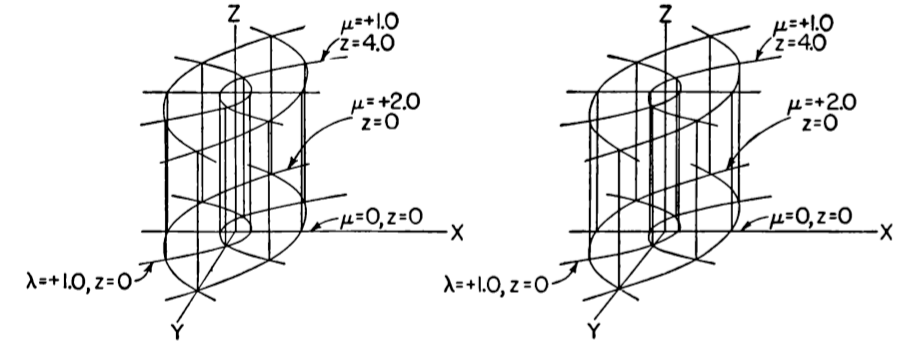
\includegraphics[scale=0.75]{Imagenes/Estereograma_01_Cilindrico_Eliptico.png}
\end{figure}
\newpage
\begin{figure}[H]
    %\hspace*{-2cm}
    \centering    
    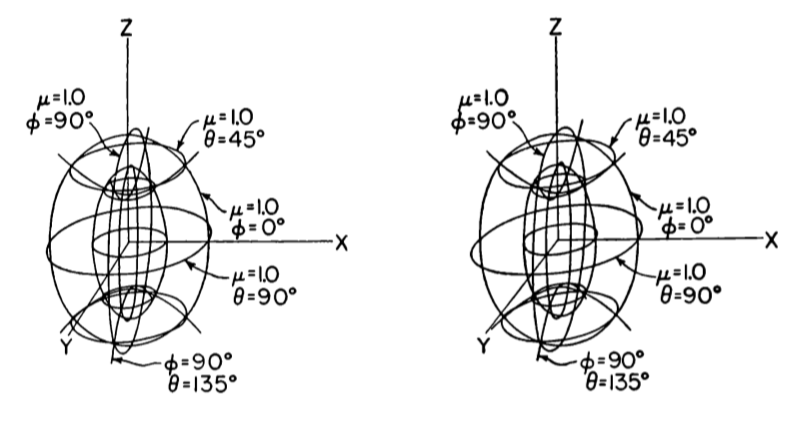
\includegraphics[scale=0.75]{Imagenes/Estereograma_02_Prolato.png}
\end{figure}
\end{landscape}
\end{document}